%% For double-blind review submission, w/o CCS and ACM Reference (max submission space)
\documentclass[sigplan,10pt,review]{acmart}\settopmatter{printfolios=true,printccs=false,printacmref=false}
%% For double-blind review submission, w/ CCS and ACM Reference
%\documentclass[sigplan,10pt,review,anonymous]{acmart}\settopmatter{printfolios=true}
%% For single-blind review submission, w/o CCS and ACM Reference (max submission space)
%\documentclass[sigplan,10pt,review]{acmart}\settopmatter{printfolios=true,printccs=false,printacmref=false}
%% For single-blind review submission, w/ CCS and ACM Reference
%\documentclass[sigplan,10pt,review]{acmart}\settopmatter{printfolios=true}
%% For final camera-ready submission, w/ required CCS and ACM Reference
%\documentclass[sigplan,10pt]{acmart}\settopmatter{}


%% Conference information
%% Supplied to authors by publisher for camera-ready submission;
%% use defaults for review submission.
\acmConference[PL'17]{ACM SIGPLAN Conference on Programming Languages}{January 01--03, 2017}{New York, NY, USA}
\acmYear{2017}
\acmISBN{} % \acmISBN{978-x-xxxx-xxxx-x/YY/MM}
\acmDOI{} % \acmDOI{10.1145/nnnnnnn.nnnnnnn}
\startPage{1}

%% Copyright information
%% Supplied to authors (based on authors' rights management selection;
%% see authors.acm.org) by publisher for camera-ready submission;
%% use 'none' for review submission.
\setcopyright{none}
%\setcopyright{acmcopyright}
%\setcopyright{acmlicensed}
%\setcopyright{rightsretained}
%\copyrightyear{2017}           %% If different from \acmYear

%% Bibliography style
\bibliographystyle{ACM-Reference-Format}
%% Citation style
%\citestyle{acmauthoryear}  %% For author/year citations
%\citestyle{acmnumeric}     %% For numeric citations
%\setcitestyle{nosort}      %% With 'acmnumeric', to disable automatic
                            %% sorting of references within a single citation;
                            %% e.g., \cite{Smith99,Carpenter05,Baker12}
                            %% rendered as [14,5,2] rather than [2,5,14].
%\setcitesyle{nocompress}   %% With 'acmnumeric', to disable automatic
                            %% compression of sequential references within a
                            %% single citation;
                            %% e.g., \cite{Baker12,Baker14,Baker16}
                            %% rendered as [2,3,4] rather than [2-4].


%%%%%%%%%%%%%%%%%%%%%%%%%%%%%%%%%%%%%%%%%%%%%%%%%%%%%%%%%%%%%%%%%%%%%%
%% Note: Authors migrating a paper from traditional SIGPLAN
%% proceedings format to PACMPL format must update the
%% '\documentclass' and topmatter commands above; see
%% 'acmart-pacmpl-template.tex'.
%%%%%%%%%%%%%%%%%%%%%%%%%%%%%%%%%%%%%%%%%%%%%%%%%%%%%%%%%%%%%%%%%%%%%%


%% Some recommended packages.
\usepackage{booktabs}   %% For formal tables:
                        %% http://ctan.org/pkg/booktabs
\usepackage{subcaption} %% For complex figures with subfigures/subcaptions
                        %% http://ctan.org/pkg/subcaption

\usepackage{graphicx}
\usepackage{graphics}
\usepackage{amsmath,amssymb, amsfonts, mathtools}
\usepackage{isabelle,isabellesym}
\usepackage{listings}

\newcommand{\defeq}{\mathrel{\stackrel{\mbox{\tiny \it def}}{=}}}
\newcommand{\subpred}{\Rightarrow}
%\newcommand{\subpred}{\mathrel{\stackrel{\cdot}{\subseteq}}}
\newcommand{\sconj}{\wedge^*}
\newcommand{\coloncolon}{\mathrel{::}}
\newcommand{\pvalid}[3]{\models\{#1\}\:#2\:\{#3\}}
\newcommand{\tvalid}[3]{\models[#1]\:#2\:[#3]}
\newcommand{\ttrip}[5]{\mathit{#1} \vdash_{\mathrm{#2}}[#3]\:#4\:[#5]}
\newcommand{\xnext}{\mathit{next}}
\newcommand{\code}[1]{\mathit{code}(#1)}
\newcommand{\cont}{\mathit{continuing}}
\newcommand{\ncont}{\mathit{not\mbox{-}continuing}}
\newcommand{\pc}{\mathit{pc}}
\newcommand{\gaspred}{\mathit{gas\mbox{-}pred}}
\newcommand{\stackh}{\mathit{stack\mbox{-}height}}
\newcommand{\stack}{\mathit{stack}}
\newcommand{\instr}[1]{\mathtt{#1}}
\newcommand{\pure}[1]{\langle#1\rangle}
\newcommand{\hd}{\mathit{head}\:}
\newcommand{\RuleL}[2]{\begin{array}{l}#1\\\hline\noalign{\smallskip}#2\end{array}}
\newcommand{\RuleC}[2]{\begin{array}{c}#1\\\hline\noalign{\smallskip}#2\end{array}}
\newcommand{\Rule}[2]{\dfrac{#1}{#2}}
\newcommand{\bblocks}{\mathit{build\mbox{-}blocks}}
\newcommand{\cblocks}{\mathit{connect\mbox{-}blocks}}
\newcommand{\fblock}{\mathit{first\mbox{-}block}}
\newcommand{\len}[1]{|#1|}
\newcommand{\wfblocks}{\mathit{wf\mbox{-}blocks}}

%%%%%%%%%%%%%%%%%%
\newcommand{\sid}[1]{\textit{\textbf{#1 [sid]}}}



% define solidity colorscheme

\lstset{
  basicstyle=\footnotesize,
  commentstyle=\rm\it,
  flexiblecolumns=false,
  breaklines=true,
  breakautoindent=false
}

% possible usage
%\lstinline!apply(simp)!
%\begin{lstlisting}[language=Isar]{}
%datatype type = IntType | BoolType | FunType type type | ErrorType
%\end{lstlisting}
%\lstinputlisting[language=Isar]{foo.thy}

% Taken from Lena Herrmann at 
% http://lenaherrmann.net/2010/05/20/javascript-syntax-highlighting-in-the-latex-listings-package
\definecolor{lightgray}{rgb}{.9,.9,.9}
\definecolor{darkgray}{rgb}{.4,.4,.4}
\definecolor{purple}{rgb}{0.65, 0.12, 0.82}

\lstdefinelanguage{Solidity}{
  keywords={typeof, new, true, false, catch, function, return, null, catch, switch, var, if, in, while, do, else, case, break, returns, contract, public},
  keywordstyle=\color{blue}\bfseries,
  ndkeywords={class, export, boolean, throw, implements, import, this},
  ndkeywordstyle=\color{darkgray}\bfseries,
  identifierstyle=\color{black},
  sensitive=false,
  comment=[l]{//},
  morecomment=[s]{/*}{*/},
  commentstyle=\color{purple}\ttfamily,
  stringstyle=\color{red}\ttfamily,
  morestring=[b]',
  morestring=[b]"
}

\lstset{
   extendedchars=true,
   tabsize=2,
   breaklines=true,
   captionpos=b
}

% end define Solidity colorscheme
% define  Isar
\lstdefinelanguage{Isar}%
  {keywords={
        theory,end,types,datatype,consts,defs,primrec,
        syntax,translations,apply,definition,fun,function, lemma,theorem,corollary,
        done,sorry,goal,proof,fixed variables, inductive, where, case,of,if,then,else,method},
        sensitive=true,
        comment=[s]{(*}{*)},
        commentstyle=\color{purple}\ttfamily,
        keywordstyle=\color{blue}\bfseries,
        literate=
                {\\<not>}{{$\<not>$}}1 {\\<times>}{{$\<times>$}}1                 
                {\\<Rightarrow>}{{$\Rightarrow$}}1%
                {\\<models>}{{$\models$}}1%
                {\\<equiv>}{{$\equiv$}}1 {~=}{{$\not=$}}1                         
                {\\<rightleftharpoons>}
                        {{$\rightleftharpoons$}}1
                {\\<exists>}{{$\exists$}}1
                {\\<parallel>}{{$\parallel$}}1
                {\\<Longrightarrow>}
                        {{$\Longrightarrow$}}1
                 {\\<lbrakk>}{{$\lsemantics$}}1
                {\\<rbrakk>}{{$\rsemantics$}}1
                {\\<longrightarrow>}
                        {{$\longrightarrow$}}1
                {\\<and>}{{$\land$}}1
                {\\<or>}{{$\lor$}}1
                {\\<bigwedge>}{{$\bigwedge$}}1
                {\\<forall>}{{$\forall$}}1
                {\\<langle>}{{$\langle$}}1
                {\\<rangle>}{{$\rangle$}}1
                {\\<union>}{{$\cup$}}1
                {ü}{"u}1 {ä}{"a}1 {ö}{"o}1
                {Ü}{"U}1 {Ä}{"A}1 {Ö}{"O}1 {ß}{{ss}}1
  }



% end define Isar



\begin{document}

%% Title information
\title[Towards Verifying Ethereum Smart Contracts]{Towards Verifying Ethereum Smart Contract Bytecode in Isabelle/HOL}         %% [Short Title] is optional;
                                        %% when present, will be used in
                                        %% header instead of Full Title.
%\titlenote{with title note}             %% \titlenote is optional;
                                        %% can be repeated if necessary;
                                        %% contents suppressed with 'anonymous'
%\subtitle{Subtitle}                     %% \subtitle is optional
%\subtitlenote{with subtitle note}       %% \subtitlenote is optional;
                                        %% can be repeated if necessary;
                                        %% contents suppressed with 'anonymous'


%% Author information
%% Contents and number of authors suppressed with 'anonymous'.
%% Each author should be introduced by \author, followed by
%% \authornote (optional), \orcid (optional), \affiliation, and
%% \email.
%% An author may have multiple affiliations and/or emails; repeat the
%% appropriate command.
%% Many elements are not rendered, but should be provided for metadata
%% extraction tools.

%% Authors with single affiliation.

%% AUTHORS APPEAR IN ALPHABETIC ORDER

\author{Sidney Amani}
%\authornote{with author1 note}          %% \authornote is optional;
                                        %% can be repeated if necessary
%\orcid{nnnn-nnnn-nnnn-nnnn}             %% \orcid is optional
\affiliation{
%  \position{Position1}
  \department{Data61}              %% \department is recommended
  \institution{CSIRO}            %% \institution is required
%  \streetaddress{Street1 Address1}
%  \city{City1}
  \state{NSW}
%  \postcode{Post-Code1}
  \country{Australia}                    %% \country is recommended
}
\email{Sidney.Amani@data61.csiro.au}          %% \email is recommended

\author{Myriam B\'egel}
\authornote{work done while at Data61, CSIRO}          %% \authornote is optional;
                                        %% can be repeated if necessary
%\orcid{nnnn-nnnn-nnnn-nnnn}             %% \orcid is optional
\affiliation{
%  \position{Position1}
%  \department{Department1}              %% \department is recommended
  \institution{\'Ecole Normale Sup\'erieure Paris-Saclay}            %% \institution is required
%  \streetaddress{Street1 Address1}
%  \city{City1}
%  \state{State1}
%  \postcode{Post-Code1}
  \country{France}                    %% \country is recommended
}
\email{Myriam.Begel@ens-paris-saclay.fr}          %% \email is recommended


\author{Maksym Bortin}
%\authornote{with author1 note}          %% \authornote is optional;
                                        %% can be repeated if necessary
%\orcid{nnnn-nnnn-nnnn-nnnn}             %% \orcid is optional
\affiliation{
%  \position{Position1}
  \department{Data61}              %% \department is recommended
  \institution{CSIRO}            %% \institution is required
%  \streetaddress{Street1 Address1}
%  \city{City1}
  \state{NSW}
%  \postcode{Post-Code1}
  \country{Australia}                    %% \country is recommended
}
\email{Maksym.Bortin@data61.csiro.au}          %% \email is recommended

\author{Mark Staples}
%\authornote{with author1 note}          %% \authornote is optional;
                                        %% can be repeated if necessary
%\orcid{nnnn-nnnn-nnnn-nnnn}             %% \orcid is optional
\affiliation{
%  \position{Position1}
  \department{Data61}              %% \department is recommended
  \institution{CSIRO}            %% \institution is required
%  \streetaddress{Street1 Address1}
%  \city{City1}
  \state{NSW}
%  \postcode{Post-Code1}
  \country{Australia}                    %% \country is recommended
}
\email{Mark.Staples@data61.csiro.au}          %% \email is recommended

%% Abstract
%% Note: \begin{abstract}...\end{abstract} environment must come
%% before \maketitle command
\begin{abstract}
Blockchain technology has increasing attention in research and across many industries.
The Ethereum block\-chain offers \emph{smart contracts}, which are small programs defined,
executed, and recorded as transactions in the blockchain transaction history.
These smart contracts run on the Ethereum virtual machine (EVM) and can be used to encode
agreements, transfer assets, and enforce integrity conditions in relationships between parties.
Smart contracts can carry financial value, and are increasingly
used for safety-, security-, or mission-critical purposes.
Errors in smart contracts have and will lead to loss or harm.
Formal verification can provide the highest level of confidence about the
correct behaviour of smart contracts.
In this paper we extend an existing EVM formalisation~\cite{Yoichi} in Isabelle/HOL by a sound
program logic at the level of bytecode.
We structure bytecode sequences into graphs of basic blocks of straight-line
code and create a program logic to reason about these.
This abstraction is a step towards control of the cost and complexity of formal verification
of EVM smart contracts.
\end{abstract}


%% 2012 ACM Computing Classification System (CSS) concepts
%% Generate at 'http://dl.acm.org/ccs/ccs.cfm'.
\begin{CCSXML}
<ccs2012>
<concept>
<concept_id>10011007.10011006.10011008</concept_id>
<concept_desc>Software and its engineering~General programming languages</concept_desc>
<concept_significance>500</concept_significance>
</concept>
<concept>
<concept_id>10003456.10003457.10003521.10003525</concept_id>
<concept_desc>Social and professional topics~History of programming languages</concept_desc>
<concept_significance>300</concept_significance>
</concept>
</ccs2012>
\end{CCSXML}

\ccsdesc[500]{Software and its engineering~General programming languages}
\ccsdesc[300]{Social and professional topics~History of programming languages}
%% End of generated code


%% Keywords
%% comma separated list
\keywords{formal verification, blockchain, smart contracts, Ethereum, Isabelle/HOL}  %% \keywords are mandatory in final camera-ready submission


%% \maketitle
%% Note: \maketitle command must come after title commands, author
%% commands, abstract environment, Computing Classification System
%% environment and commands, and keywords command.
\maketitle


\section{Introduction}
\label{sec:intro}
Blockchain technology emerged to support financial transactions in the Bitcoin system, but has become
increasingly important in many industries, with potential use in legal, medical, and
supply chain industries.
The Ethereum blockchain provides a general-purpose computational mechanism called \emph{smart contracts}.
These are programs that run on the Ethereum virtual machine~\cite{wood2014ethereum} (EVM), and
are recorded in the blockchain history.  They can be used to encode or execute agreements between parties.
For example, a party invoking a smart contract could cause digital currency to be transferred to another
party, or could record a state change which makes the other party eligible to invoke other transactions.
Smart contracts provide new ways to implement multi-party relationships within blockchain-based applications.
In addition to the direct financial value in these applications, blockchains are increasingly being
used for safety-critical applications such for pharmaceutical supply chains, or for mission-critical
application such as in electrical power grids.
We must know that smart contract implementations do not violate critical requirements, and
formal modelling and verification can be applied in this context.
%
To address these questions we seek:
\begin{itemize}
\item[(i)] a trustworthy logical framework capable of expressing complex safety and security
   requirements; 
\item[(ii)] a valid formal model of the EVM within the framework; 
\item[(iii)] a sound program logic defined within the framework able to
reason about properties of smart contracts. 
\end{itemize}
In our setting, we use the logical framework Isabelle/HOL, and an existing EVM formal
model~\cite{Yoichi}.
Thus, our remaining goal is a sound program logic.  In this paper we propose such a logic for EVM bytecode. 
We target unstructured bytecode rather than a high-level programming language for several reasons.
Firstly, our approach is independent of high-level languages (e.g.\ Solidity) and their compilers, which
makes our work more general and significantly less reliant
on the correctness of higher-level tools.
Secondly, bytecode is the actual programming language of Ethereum as all smart contracts appear only
in this form on the blockchain.
Thus we target EVM bytecode, despite the necessity for us to restore structures (such as conditionals)
that we might take for granted in higher-level languages.
We describe our approach for this in the remainder of the paper. 

The main contributions of the paper are:
\begin{itemize}
\item[(i)] an extension to the EVM formalisation~\cite{Yoichi} in the Isabelle/HOL theorem prover,
           covering smart contract correctness properties, and which gives a separate universal
           treatment of termination based on Ethereum's concept of execution `gas';
\item[(ii)] a sound program logic to verify smart contracts at the bytecode level; and
\item[(iii)] Isabelle tactics to support automated generation of verification
            conditions using the rules of the logic.
\end{itemize}
         
The paper is structured as follows. Section~\ref{sec:bg} describes the background
for the presented work. Section~\ref{sec:corr} describes how we can capture correctness properties in a pre/postcondition
style for EVM bytecode programs. Section~\ref{sec:logic} is devoted to our program logic, 
%i.e. rules for generation of verification conditions out of a contract, 
whereas Section~\ref{sec:sound} shows the soundness of the logic
w.r.t. the correctness property.
Section~\ref{sec:case} presents a case-study, where we outline the
specification and verification of real bytecode, as well as how
we automate generation of verification conditions using Isabelle tactics.
Finally, Section~\ref{sec:rwork} outlines some related work and
Section~\ref{sec:concl} summarises the results and gives an outlook.
%
\section{Background} 
\label{sec:bg}
The EVM is described in the Ethereum `Yellow Paper'~\cite{wood2014ethereum}.
This provides a clear foundation not only for its implementation, but also for its formalisation in logic.
One such formalisation has been provided~\cite{Yoichi} using the `meta-tool' \emph{Lem}~\cite{DBLP:conf/icfp/MulliganOGRS14}.
Lem supports a variety of theorem provers including Isabelle/HOL.
\emph{Isabelle}~\cite{Nipkow_PW:Isabelle} is a logical framework and interactive generic theorem prover.
Isabelle/HOL encodes higher-order logic and is the most important and most developed logic in Isabelle.
Isabelle's LCF-style architecture,
based on a small (meta)-logical inference kernel, provides very high confidence about its sound
implementation as a theorem prover.
 
The EVM formalisation needs to be validated to provide confidence that the formal model
and EVM implementations coincide. To this end, a validation test suite accompanies
the model in Lem. Using this, EVM implementations and OCaml code generated by Lem from the EVM
formal model are both applied to a large collection of contracts, cross-checking their outputs.  

We entirely focus on the EVM model in Isabelle/HOL, so additionally run the test suite 
on OCaml code generated by Isabelle. This our `double-validation' 
process as outlined in Figure~\ref{fig:valid}.          
\begin{figure}[htbp]
\centering
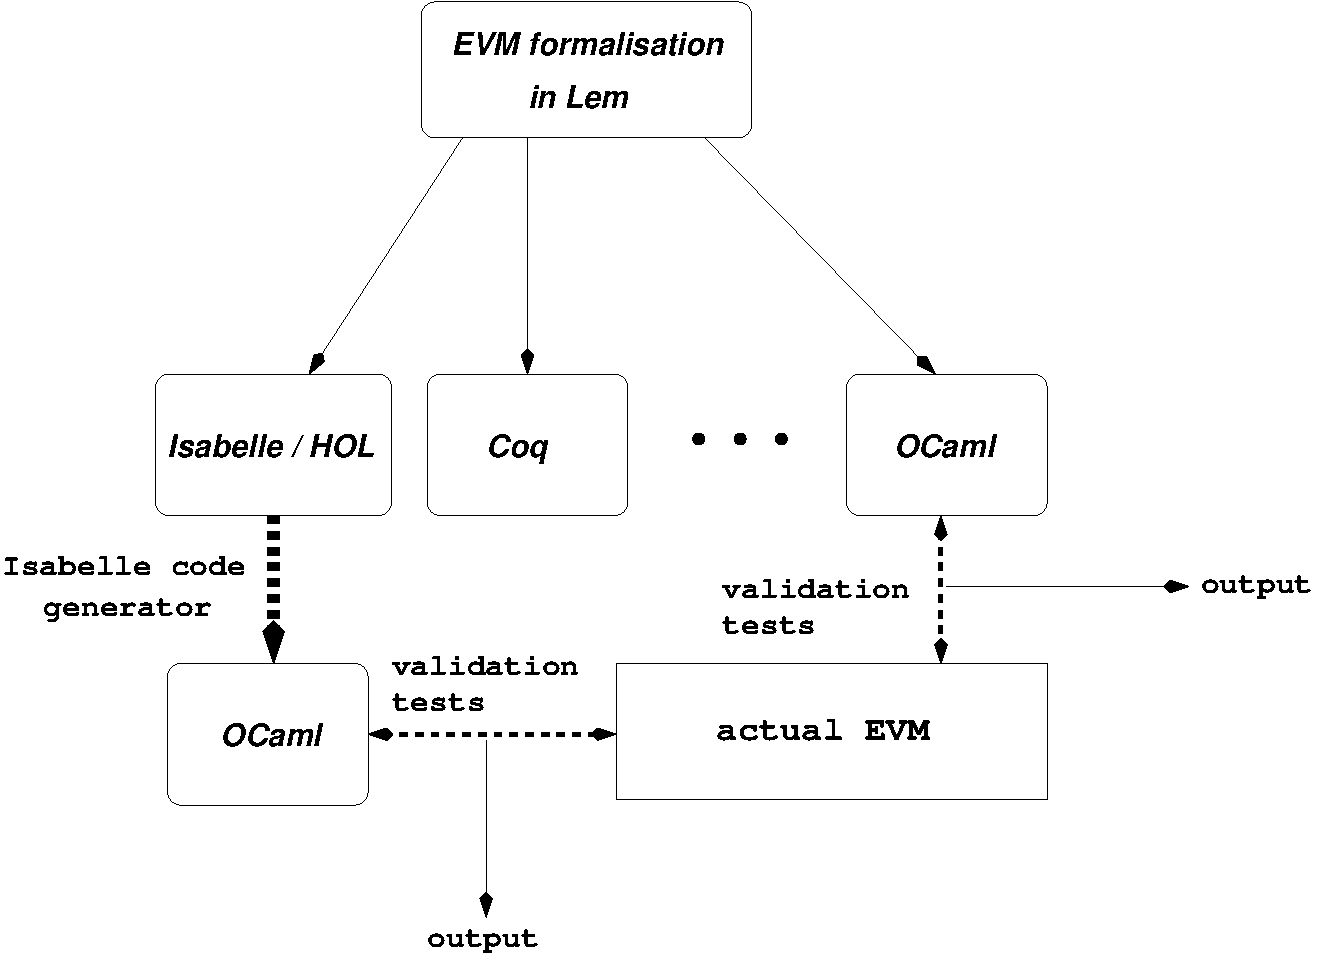
\includegraphics[height=5.5cm, width=7.5cm]{images/evm_lem}    
        \caption{Validation of EVM models}
\label{fig:valid}
\end{figure}
The use of the test suite from Isabelle has required certain efforts, mainly because 
of different representations of machine words. OCaml code from Lem uses efficient native modules,
whereas the Isabelle side invokes a formally-verified theory of machine words.
Because of this, our suite needs much more time to pass the tests.
Nonetheless, we gain a complementary indication that all three models of EVM follow the specification
and behave equally.    
%
\section{Total Correctness of EVM Bytecode Programs}
\label{sec:corr}
In his PhD thesis~\cite{DBLP:phd/ethos/Myreen09}, Myreen introduced a general 
method of formal 
machine code verification with a particular application to ARM. In this section we show how
this general method can be adapted to EVM, taking however additional accounts of the EVM specific properties rooted in the 
gas consumption.
 
In the general model, a state carries all the information needed to execute a program, including
instructions (with respective reference numbers) constituting the program itself, a program counter that
refers to the current instruction, a stack and so on. All these elements are treated uniformly 
as sets of so-called \emph{state elements}
and separated in a state using separation logic conjuncts $\sconj$~\cite{Reynolds_02}.  
Then a single machine step can be captured by a function $\xnext$ that 
takes the current instruction and transforms the state in accordance with the instructions
specified behaviour. Of course, $\xnext$ might not always be able to pick an instruction
as an execution can have terminated properly or with an exception. This is indicated within a state
by the $\ncont$ flag, which is just an abbreviation for the state element 
$\mathit{ContinuingElm}\:False$. If $\ncont$ is present in a state, $\xnext$
leaves the state unchanged.   
   
An input/output property of a program $c$ is captured by a triple
$\pvalid{P}{c}{Q}$, where $P$ and $Q$ are separation logic predicates on the state.
The triple is true iff for any state $s$ and frame $F$ such that
$(P \sconj \code{c} \sconj F)\:\ s$ holds, there exists a natural number $k$ such that 
$(Q \sconj \code{c} \sconj F)\:\ \xnext^k(s)$ holds. 
%The frame is used to accomodate an invariant part of a state, 
Keeping frame $F$ will allow us to reason about parts of states locally, %using \emph{frame rule}(cf.~\cite{Reynolds_02}),
whereas $\xnext^k$ denotes $k$-times iteration of $\xnext$.
Such triples $\pvalid{P}{c}{Q}$ are highly generic and we cannot conclude much from many of these, except that
under given preconditions the program $c$ will pass a state satisfying $Q$. This changes immediately in cases when $Q$ is of
the form $\ncont \sconj Q'$, now stating that $c$ has reached a terminating state satisfying $Q'$.
Hence, showing $\pvalid{P}{c}{\ncont \sconj Q'}$ amounts to showing termination of the program $c$ in
a $Q'$-state.

This generic technique applies seamlessly to EVM programs as
the formalisation~\cite{Yoichi} shows.
However, we realised that showing termination of a contract individually is an unnecessary burden because
Ethereum was designed in such a way that all smart contracts
are guaranteed to terminate (either successfully or due to an `out-of-gas' exception).
More specifically, to ensure that miners get compensated for the electricity cost
incurred by running smart contracts, each EVM instruction
has a gas fee.
Thus, when invoking a contract, the initiator provides a gas budget
proportional to how computationally expensive the execution is expected
to be and every step of execution is deducted from the budget.
If the gas consumption exceeds the budget, an `out-of-gas' exception is
raised and the state of the contract prior the
invocation is restored.

These blockchain specifics give us a termination order we need   
to augment the EVM formalisation~\cite{Yoichi} by the function $\xnext^*$ which 
consequently assigns to each state the terminal element from the reflexive-transitive closure of $\xnext$. 
The essential property of $\xnext^*$ is that for any state $s$ there exists $k \geq 0$ such that
\begin{itemize}
\item[(i)] $\xnext^*(s) = \xnext^k(s)$
\item[(ii)] $\xnext^l(s)$ can continue for any $l$ such that $0 \le l < k$
\item[(iii)] $\xnext^l(s)$ cannot continue for any $l \ge k$.
\end{itemize}
In other words, $\xnext^*(s) = \xnext^k(s)$ where $k$ is the least number such that
$\xnext^k(s)$ reaches a state with $\ncont$. 
% Perhaps say that we proved that every program in EVM bytecode terminates by writing
% higher-order logic function that executes bytecode (reusing Yoichi's definitions of
% semantics) and proving termination of that function.

Now, regarding the contract correctness, we strengthen $\pvalid{P}{c}{Q}$ to 
a total correctness property $\tvalid{P}{c}{Q}$ which is consequently true iff
for any state $s$ and frame $F$ 
$(P \sconj \code{c} \sconj F)\: s$ implies $(Q \sconj \code{c} \sconj F)\: \xnext^*(s)$. 
To sum up, what we achieved so far is to factor out the termination part which we have 
shown \emph{once and for all} contracts, thus removing this obligation from the verification
process completely. In the next section we will present our program logic handling EVM bytecode, 
which (based on soundness presented in Section~\ref{sec:sound}) will give us 
a sound device to derive verification conditions for contract properties of the form $\tvalid{P}{c}{Q}$.   
%       
\section{Program Logic}
\label{sec:logic}
A Hoare-style program logic comprises a collection of rules that allow us to derive semantic properties 
of compound programs from properties of its parts. In case of structured languages 
we usually have, for instance, a rule telling us that a program \textbf{if} $C$ \textbf{then} $p_1$ \textbf{else} $p_2$
exhibits a certain input/output behaviour if $p_1$ and $p_2$ do so, however, with the additional precondition $C$ 
available for $p_1$ and $\neg C$ for $p_2$.
However, the situation is not that simple when we have to deal with
unstructured programs like EVM bytecode in our case.
In such setting, the aforementioned conditional compound constructs
appear merely as jump instructions that transfer the flow of execution
to another part of the program.
Since a bytecode program comprises
a list of instructions, a rule might handle the head instruction and proceed to the tail of 
the list, but would need to make exceptions when the head instruction is a jump, because then
the tail does not necessarily correspond to the next instructions in the flow of execution.
Although such treatment is in principle possible,
there are more sophisticated decompilation techniques available, such as extraction of 
\emph{Control Flow Graphs} (CFG), in particular applied to the Java Virtual Machine (JVM) code~\cite{zhao99}.
The aim of CFG extraction is to split a program into \emph{basic blocks}, i.e. sequences of
instructions without jumps, and connect them
using edges corresponding to jumps.
The essential property of basic blocks is that
it comprises straight-line code, i.e. the execution always enters it at its first instruction
and leaves only after the last one has been executed.

However, the algorithm to compute the edges of a CFG for JVM bytecode
cannot be easily adapted to our EVM context.
This is because JVM jump instructions
take their target address as an immediate value argument which can be determined statically,
whereas in EVM jump destinations
must be obtained from the stack, i.e. dynamically. For that reason, our bytecode preprocessing
currently addresses basic block extraction only, presented in the next section.
Then, Sections~\ref{sec:prog-rules}, \ref{sec:block-rules} and \ref{sec:instr-rules} 
present how our logic handles programs, splitted into blocks, individual blocks, and
instructions within blocks, respectively. 
%
%       
%The basic blocks program logic we present in this section is organised
%in three levels of inductively defined inference rules, of the form:
%\[
%\begin{array}{l}
%\ttrip{\mathit{blocks}}{\mathtt{prog}}{P}{(n, \mathit{xs}, t)}{Q} \\
%\ttrip{}{\mathtt{block}}{P}{\mathit{xs}}{Q} \\
%\ttrip{}{\mathtt{instr}}{P}{\mathit{x}}{Q} 
%\end{array}
%\]
%where $P, Q$ are state predicates,
%$\mathit{blocks}$ is a list of basic blocks,
%$(n, \mathit{xs}, t)$ is a basic block,
%$\mathit{xs}$ is a list of instructions,
%and $x$ is an instruction.
%
%The program level allows considering one basic block at a time.
%The block level, one instruction at a time.
%And the instruction level provides rules for every instruction defined on the EVM.
%In the rest of this section we first explain in detail how we
%split EVM bytecode into basic blocks, then we dedicate a section to
%each level of the program logic.
%
\subsection{Extraction of Basic Blocks}
We divide instructions into three groups:
\begin{itemize}
\item[(i)] $\instr{JUMPDEST}$ indicates a jump destination and hence beginning of a
                                 basic block;
\item[(ii)] $\instr{JUMP}$, $\instr{JUMPI}$, $\instr{UNKNOWN}$ and all of 
            \emph{Misc}-instructions\footnote{RETURN, STOP, SUICIDE, CREATE, CALL, CALLCODE, DELEGATECALL}
            indicate the end of a basic block ($\instr{UNKNOWN}$ and Misc-instructions interrupt program execution); 
\item[(iii)] all remaining instructions that form the contents of basic blocks.
\end{itemize}  
Furthermore, we classify basic blocks by means of the following four types:
\begin{itemize}
\item[(i)] \textit{Terminal} -- if the last instruction of the block interrupts execution;
\item[(ii)] \textit{Jump} -- if the last instruction is $\instr{JUMP}$;
\item[(iii)] \textit{Jumpi} -- if the last instruction is $\instr{JUMPI}$;
\item[(iv)] \textit{Next} -- otherwise, i.e. when control passes from the last instruction of the block
                             to the instruction with the successor address.                         
\end{itemize} 
Figure~\ref{fig:basicblocks} illustrates how we split EVM bytecode into basic blocks of different
types, thereby indexing the blocks with addresses of their first instruction
and removing all the jumps from the list of instructions.
The entire extraction process is captured in Isabelle
by the function $\bblocks$ which maps a list of instructions to a list of tuples $(i, \mathit{xs}, t)$,
where $i$ is the block index, $\mathit{xs}$ --- the list of instructions of the block, and $t$ --- the type of
the block. 

By splitting bytecode into basic blocks no information gets lost since we can connect the produced blocks
in the right order and insert jumps back in accordance with block types. More precisely, we also have the function
$\cblocks$ such that for any bytecode program $c$ the identity 
\[\cblocks(\bblocks\:c) = c\] holds.  
\begin{figure}
\center
\begin{tabular}{c r l c}
                block index & address & instruction & block type\\
                        \hline
                &       0       &       $\instr{OR}$&\\
                &       1       &       $\instr{ADD}$&\\
                {0}&    2       &       $\instr{SWAP1}$&  \textit{Next}\\
                        \hline
                &       3       &       $\instr{JUMPDEST}$&\\
                &       4       &       $\instr{MLOAD}$&\\
                &       5       &       $\instr{POP}$&\\
                {3}&    \textcolor{gray}{6}     &       {\color{gray}$\instr{JUMP}$}& \textit{Jump}\\
                        \hline
                &       7       &       $\instr{DUP3}$&\\
                &       8       &       $\instr{PUSH}\;0$&\\
                &       10      &       $\instr{ISZERO}$&\\
                {7}&    \textcolor{gray}{11}    &       {\color{gray}$\instr{JUMPI}$}& \textit{Jumpi}\\
                        \hline
                &       12      &       $\instr{POP}$&\\
                {12}&   13      &       $\instr{RETURN}$& \textit{Terminal}\\
                        \hline
        \end{tabular}
\caption{A program split into basic blocks, where grey instructions appear in the original
         code but are removed from the list of instructions of their block.}
\label{fig:basicblocks}
\end{figure}

Based on these preparations, the following predicates 
\[
\begin{array}{l}
\ttrip{}{\mathtt{instr}}{P}{\mathit{x}}{Q} \\
\ttrip{}{\mathtt{block}}{P}{\mathit{xs}}{Q} \\
\ttrip{\mathit{blocks}}{\mathtt{prog}}{P}{(n, \mathit{xs}, t)}{Q}
\end{array}
\]
where $P, Q$ are state predicates, $x$ --- an instruction, $\mathit{xs}$ --- a list of instructions,
$\mathit{blocks}$ --- a list of basic blocks, and
$(n, \mathit{xs}, t)$ --- a basic block, are defined inductively in the following three sections.
%
\subsection{Program Rules}
\label{sec:prog-rules}
%
We start at the program level, where we have the following rules for
each case of the block type $t$.
\[
\begin{array}{l l}
\mbox{(i)} & \RuleC{\ttrip{}{\mathtt{block}}{P}{\mathit{xs}}{Q}}
     {\ttrip{\mathit{blocks}}{\mathtt{prog}}{P}{(n, \mathit{xs}, \mathit{Terminal})}{Q}}
\end{array}
\]
That is, a $\mathit{Terminal}$-block is simply passed to the level of
blocks as we do not need to look at any other block after this has been processed.  

The rule for a $\mathit{Next}$-block is different in this sense:
\[
\begin{array}{l l}
\mbox{(ii)} & \RuleC{\begin{array}{l} \ttrip{}{\mathtt{block}}{P}{\mathit{xs}}{\pc\;m \sconj R} \\
                                      (m, \mathit{ys},t) \in \mathit{blocks} \\
                                       \ttrip{\mathit{blocks}}{\mathtt{prog}}{\pc\;m \sconj R}{(m, \mathit{ys},t)}{Q}
                     \end{array}}
     {\ttrip{\mathit{blocks}}{\mathtt{prog}}{P}{(n, \mathit{xs}, \mathit{Next})}{Q}}
\end{array}
\]
The state element $\pc\;m$ determines the program counter after $\mathit{xs}$ has been
processed. Then we need to retrieve the next block associated to the index $m$ from the structure $\mathit{blocks}$,
which is expressed by $(m, \mathit{ys},t) \in \mathit{blocks}$, and proceed with 
$(m, \mathit{ys},t)$.

Further, in case of a $\mathit{Jump}$-block we additionally need to retrieve the address of the jump 
destination from the stack 
after the block has been processed. This yields the following, slightly more involved, rule:
\[
\begin{array}{l l}
\mbox{(iii)} & \RuleC{\begin{array}{l}\ttrip{}{\mathtt{block}}{P}{\mathit{xs}}{R_1} \\
                                      (j, \mathit{ys},t) \in \mathit{blocks} \\
                                      \hd\mathit{ys} = (j, \instr{JUMPDEST}) \\
                                      \ttrip{\mathit{blocks}}{\mathtt{prog}}{R_2}{(j, \mathit{ys},t)}{Q}
                      \end{array}}
     {\ttrip{\mathit{blocks}}{\mathtt{prog}}{P}{(n, \mathit{xs}, \mathit{Jump})}{Q}}
\end{array}
\]
where $R_1$ and $R_2$ abbreviate the conditions \\
\\$
\begin{array}{l}
\pure{h \le 1023 \wedge g \geq 8} \sconj \cont \sconj \gaspred\:g \; \sconj \\
\pc\:i \; \sconj \stackh\:(h + 1) \sconj \stack\:h\:j \sconj R 
\end{array}
$\\ 
\\
and\\
\\$
\begin{array}{l}
\cont \sconj \gaspred\:(g - 8) \; \sconj \\
\pc\:j \; \sconj \stackh\:h \sconj R 
\end{array}
$\\
\\respectively. 
Regarding the stack, $\stackh\:(h + 1)$ and $\stack\:h\:j$ specify a state where
index $h$ refers to the top of the stack containing $j$ -- the jump destination we are looking for. 
Regarding gas, $\gaspred\:g$
binds the available amount of gas to $g$, whereas 
the part $\pure{h \le 1023 \wedge g \geq 8}$ is a \emph{pure} condition,
i.e. not dependent on state, and sets an upper bound for the height of
the stack and a lower bound for the amount of gas, namely $8$ units: 
as much as EVM requires to perform a jump, which is deducted by $\gaspred\:(g - 8)$.   
Notice, that here and in the rules below we need to carry the $\cont$ state element because the EVM model~\cite{Yoichi}
imposes having either $\cont$ or $\ncont$ in a state to process instructions.
%Although the pure part is quite plain in this case, it generally allows us to express elaborated 
%conditions on state elements by means of higher-order logic formulae.      

The case of a conditional jump. i.e. a $\mathit{Jumpi}$-block, is similar, except
that we also need to retrieve from the stack the value $c$ to be compared to $0$ and
jump only if $c \neq 0$:
\[
\begin{array}{l l}
\mbox{(iv)} & \RuleC{\begin{array}{l l}\ttrip{}{\mathtt{block}}{P}{\mathit{xs}}{R_1} & \\
                                       (j, \mathit{ys},t) \in \mathit{blocks} & \\
                                       (i, \mathit{zs},t') \in \mathit{blocks} & \\
                                       \hd\mathit{ys} = (j, \instr{JUMPDEST}) & \\
  \ttrip{\mathit{blocks}}{\mathtt{prog}}{R_2}{(j, \mathit{ys},t)}{Q} & \bullet\; \mbox{if } c \neq 0 \\
  \ttrip{\mathit{blocks}}{\mathtt{prog}}{R_3}{(i, \mathit{zs},t')}{Q} & \bullet\; \mbox{if } c = 0 
                      \end{array}}
     {\ttrip{\mathit{blocks}}{\mathtt{prog}}{P}{(n, \mathit{xs}, \mathit{Jumpi})}{Q}}
\end{array}
\]  
where $R_1, R_2, R_3$ abbreviate the conditions \\
\\$
\begin{array}{l}
\pure{h \le 1022 \wedge g \geq 10} \sconj \cont \sconj \gaspred\:g \; \sconj \\
\pc\:(i - 1) \; \sconj \stackh\:(h + 2) \; \sconj \stack\:(h+1)\:j\; \sconj \\
 \stack\:h\:c \;\sconj R 
\end{array}
$\\ 
\\
and\\
\\$
\begin{array}{l}
\cont \sconj \gaspred\:(g - 10) \; \sconj \\
\pc\:j \; \sconj \stackh\:h \sconj R 
\end{array}
$\\
\\
and\\
\\$
\begin{array}{l}
\cont \sconj \gaspred\:(g - 10) \; \sconj \\
\pc\:i \; \sconj \stackh\:h \sconj R 
\end{array}
$\\
\\respectively. 
%
\subsection{Block Rules}
\label{sec:block-rules}
At the level of basic blocks we need only two simple rules
that handle the cases of non-empty and empty lists of instructions
to be processed:
\[
\begin{array}{l l}
\mbox{(i)} & \RuleC{\begin{array}{l}\ttrip{}{\mathtt{instr}}{P}{x}{R} \\
                    \ttrip{}{\mathtt{block}}{R}{\mathit{xs}}{Q}
                    \end{array}}
                   {\ttrip{}{\mathtt{block}}{P}{x\mbox{::}\mathit{xs}}{Q}}
\end{array}
\]
and
\[
\begin{array}{l l}
\mbox{(ii)} & \RuleC{P \subpred Q} 
{\ttrip{}{\mathtt{block}}{P}{\mathit{Nil}}{Q}}
\end{array}
\]
where $P \subpred Q$ means $P\:s$ implies $Q\:s$ for any state $s$.
%
\subsection{Instruction Rules}
\label{sec:instr-rules}
As we need to provide a rule for each of 70 EVM instructions, we will not
present all of them here\footnote{We presently have
proved the soundness of 30 commonly used instructions but
we expect the missing instructions to follow a similar proof structure.}.
The following rule for $\instr{POP}$ is quite representative
and shows that in the precondition we specify the necessary conditions for 
the instruction to be performed by the EVM and in the postcondition -- 
the effect of the operation on state elements:
\[
\ttrip{}{\mathtt{instr}}{P}{(n, \instr{POP})}{Q}
\]
where $P$ stands for 
\\
\\$
\begin{array}{l}
\pure{h \le 1023 \wedge g \geq 2} \sconj \cont \sconj \gaspred\:g \; \sconj \\
\pc\:n \; \sconj \stackh\:(h + 1) \; \sconj \stack\:h\:x \sconj F 
\end{array}
$\\ 
\\
and $Q$ for\\
\\$
\begin{array}{l}
\cont \sconj \gaspred\:(g - 2) \; \sconj \\
\pc\:(n+1) \; \sconj \stackh\:h \sconj F
\end{array}
$\\
\\
In particular, we have stated that the height of the stack decreases by $1$ as
an effect of $\instr{POP}$. It is also worth noting that we incorporate frames
into such instruction-specific rules by carrying a variable $F$ in pre- and
postconditions, as shown above. This is in contrast to the more common way
introducing a generic \emph{frame} rule (cf.~\cite{Reynolds_02}) of the form
\[
\RuleC{\ttrip{}{\mathtt{instr}}{P}{i}{Q}}{\ttrip{}{\mathtt{instr}}{P \sconj F}{i}{Q \sconj F}}
\] 
and removing $F$ from all instruction-specific rules. However, this treatment leads to 
a considerable overhead in the verification process, since we would need to apply
the frame rule basically each time an instruction-specific rule needs to be applied. 
%For this practical reason we omit an explicit frame rule. 

Apart from the frame rule we still have two generic rules at the instruction level:
\[
\begin{array}{l l}
\mbox{(i)} & \RuleC{\begin{array}{l}
                     \ttrip{}{\mathtt{instr}}{P'}{i}{Q'} \\
                     P \subpred P' \\ 
                     Q' \subpred Q
                     \end{array}}{\ttrip{}{\mathtt{instr}}{P}{i}{Q}}
\end{array}
\]
\[
\begin{array}{l l}
\mbox{(ii)} & \ttrip{}{\mathtt{instr}}{\pure{\mathit{False}}}{i}{Q} 
\end{array}
\]
The rule (i) is the usual `consequence' rule, allowing us to adjust pre- and
postconditions, whereas (ii) is needed to discharge trivial 
proof obligations having unsatisfiable preconditions. Such obligations 
arise frequently from conditional jumps (rule (iv), Section~\ref{sec:prog-rules})
where the condition is fully evaluated prior to the actual jump, such that
we need to follow only one of the emerging branches.

The following section puts the program logic and the results of Section~\ref{sec:corr}
together by means of a soundness proof. 
%
\section{Soundness}
\label{sec:sound}
In this context, the ultimate soundness goal comprises the proposition
\[
\RuleC{\begin{array}{l}
       0 < \len{c} < 2^{256} \\
       \ttrip{\bblocks\: c}{prog}{P}{\fblock}{Q}
       \end{array}}
{\tvalid{P}{c}{Q}}
\]
where $\fblock$ is a shorthand for the first block in $\bblocks\: c$, and
the assumption $0 < \len{c} < 2^{256}$ is necessary to avoid dealing with empty programs
as well as with programs that have more than $2^{256}$ instructions which is imposed by 
the design of EVM. In other words, to show an input/output property specified by 
$\tvalid{P}{c}{Q}$, we can transform $c$ into its basic blocks, pick the first one, and
apply the rules of our program logic to establish the property.

\section{Case-study}
\label{sec:case}

%To demonstrate the practicality of our program logic, we verify a smart contract.

% We provide the ground work to eventually get fully verified
% smart contracts. They will require reasoning about bytecode.
% Our framework could be used to have a formal connection
% between a  more structured language and bytecode.

Our framework provides the ground work for full functional correctness
of Ethereum smart contracts.
Ethereum smart contracts are typically implemented in a language called Solidity,
which provides a high level abstractions to facilitate interactions between EVM
program.
In Solidity, the functionality of a smart contract is encapsulated into a
\textit{contract interface}, which, analogously to a class in object oriented programming
(OOP), has a well-defined interface with public and private elements.
Creating a contract on the blockchain instantiates the contract interface.
Just like class instantiations in OOP, contracts on the blockchain are
stateful objects, where the storage is persistent across method function calls.

\begin{figure}[h!]
\begin{lstlisting}[language=Solidity]{}
contract MyContract {
  function dispatch1() public returns (uint) {
  	return (1);
  }
  function dispatch2() public returns (uint) {
  	return (2);
  }
}
\end{lstlisting}
\caption{Contract with two functions: \textit{dispatch1} that returns 1; \textit{dispatch2} that returns 2.}
\label{solidity}
\end{figure}

\autoref{solidity} shows an example of Solidity contract with two public functions.
Each public function of a contract gets assigned a unique hash and
the Solidity compiler produces EVM bytecode with a single entry point.
At the beginning of the bytecode a \textit{dispatcher} is introduced that inspects the first arguments
passed when the contract gets invoked, compares it with the function hashes and
calls the appropriate function.
The binary format for computing function hashes and packing arguments is standardised
in an ABI (abstract binary interface), enabling interoperability between
contracts implemented using various EVM languages.

Since the contract abstraction is provided by the Solidity language,
it is the job of the compiler to implement the dispatcher.
This means that the code can only be verified at the level of bytecode,
hence it is a great application to showcase our framework.
In this case study we show how we specified and verified the
dispatcher produced for the code in \autoref{solidity}.
%

\subsection{Specification}

\begin{figure}[h]
\begin{lstlisting}[language=Isar]{}
definition 
  spec_MyContract ::"32 word \<Rightarrow> contract_action"
where
  "spec_MyContract z = 
	(if z = dispatch1_hash 
	then ContractReturn (word_rsplit 1))
	else (if z = dispatch2_hash 
	then ContractReturn (word_rsplit 2))
	else ContractFail [ShouldNotHappen]))"

theorem verify_dispatcher:
"\<exists>r. \<models> [pc 0 \<and>* stack_height 0 \<and>*
             sent_data (word_rsplit arg) \<and>*
             sent_value 0 \<and>* memory_usage 0 \<and>*
             continuing \<and>* gas_pred 3000 \<and>* ...]
        (build_blocks bytecode_MyContract)
        [action (spec_MyContract arg) \<and>* r]"
\end{lstlisting}
\caption{Specification and functional correctness theorem of MyContract.}
\label{spec}
\end{figure}

\autoref{spec} shows our handwritten specification of \textit{MyContract} in Isabelle/HOL.
The Solidity compiler can print a contract ABI description which includes the
signatures of all public functions as well as their hashes.
We used this feature to obtain \textit{dispatch1\_hash} and \textit{dispatch2\_hash}.
The rest of the specification is straightforward.
The argument passed to \textit{spec\_MyContract} corresponds to the first 32-bit
machine word passed as argument when the contract get invoked.
\textit{ContractReturn} and \textit{ContractFail} specify the action
resulting from the contract execution.
Upon successful execution, contracts return a byte array,
hence we use \textit{word\_rsplit} to convert a word into list of bytes
encoded in big-endian format.
When none of the function hashes match the first contract argument,
the dispatcher hits an \textit{INVALID}\footnote{INVALID is the mnemonic
of an EVM opcode intentionally kept undefined in order to raise an exception.} instruction,
which corresponds to raising a \textit{ShouldNotHappen} exception
in our bytecode semantics.

At the bottom of \autoref{spec} is a Hoare triple we proved.
The precondition initialises the machine state, e.g. program counter is zero,
stack is empty, etc. Importantly, \textit{arg} is the 32-bit word contract
argument used by the dispatcher code as well as the specification,
and $\gaspred$ specifies the gas budget for the contract execution.
\textit{bytecode\_MyContract} is a list of deeply embedded EVM
instructions which we convert into a list of basic blocks with $\bblocks$.
In the postcondition, we are only interested in the resulting action
satisfying \textit{spec\_MyContract}, hence we quantify existentially
on the rest of the state to leave it unspecified.

\subsection{Verification}


Smart contract bytecode is divided into two sections: the pre-loader and
runtime code.
The pre-loader bootstraps the contract by deploying it on the
Ethereum network and running its constructor (\autoref{solidity}
has no constructor).
The runtime code contains the core functionality of the contract
that can be invoked by other blockchain agents.
Our verification only consider the runtime code of MyContract.

We obtain the runtime code as a byte string of opcode from the Solidity
compiler and convert it into a list of EVM instructions via a
Isabelle/HOL function we wrote.
In this sense we work directly on the bytecode output of
the Solidity compiler.

MyContract bytecode has 227 EVM instructions, that get split into 27 basic
blocks, including 4 of type conditional jump.
Proving the correctness of the bytecode was fairly straightforward
once the automation described in the next section reached maturity.

A difficult proof arose when parsing the contract input data
in order to extract the argument passed to the dispatcher.
This involved dealing with operations on words of different size,
which is notoriously hard.
In particular, the instruction \textit{CALLDATALOAD} reads a
256-bit machine word from the input data array.
Since the hash value passed in the input data is only a 32-bit word,
the dispatcher does the following word arithmetic to convert the value:\\
$w32\_hash = (w256\_input\_data >> 224)\ \&\ \mathtt{0xffffffff}$.\\
We had to prove that when the hash is packed in the input data,
the above bit-wise operations return the same hash value.

%% mole $ wc -l HoareTripleForBasicBlocks.thy SoundnessForBasicBlocks.thy ../example/Dispatcher.thy ../EvmFacts.thy Hoare.thy
%%    575 HoareTripleForBasicBlocks.thy
%%   2733 SoundnessForBasicBlocks.thy
%%    762 ../example/Dispatcher.thy
%%    300 ../EvmFacts.thy
%%   1077 Hoare.thy
%%   5447 total

The total development of our framework is $\approx$5000 lines of Isabelle/HOL,
excluding the existing EVM bytecode semantics, etc.
The size of the top-level specification of MyContract is $\approx$15 lines
and the functional correctness proof of the dispatcher is
$\approx$50 lines of proof specific to this example, which compares
favouribly with the $\approx$500 lines of reusable proof
automation machinery we developed.
We describe this automation next.



% focus on runtime binary, 
% parse_bytecode 
% derivation tree for bytecode, 
% word proofs

% due to hash_in_w256 being padded with zeros,
% we need to prove hash_in_w32 = (hash_in_w256 >> 224) & 0xffffffff
% >> 224 removes the padded zeros
% Word proofs are notorious to be hard and this was one of them.

\subsection{Automation}
% Ideas: show isabelle tactics,
% number of lines of proofs

When reasoning about bytecode, even the verification of small smart contracts
can involve long, tedious and repetitive proofs.
Hence, our program logic was purposefully designed to be
amenable to proof automation.

The inductively defined inference rules presented in \autoref{sec:logic}
are all designed to be used in a syntactically-driven verification
condition generator (VCG).
Shaping the rules in a way that only one of them applies at each point in the
proof makes it trivial to write a VCG that merely tries applying all the rules
one after another.
Such VCG can be implemented with a few lines of Eisbach~\cite{Matichuk_MW_16}---
an Isabelle/HOL's high-level tactic language.
We developed a VCG for each level of our program logic.
For instance, the program-level tactic looks like this:
\begin{lstlisting}[language=Isar]{}
method prog_vcg =
 (prog_jumpi_vcg | prog_jump_vcg
 | prog_terminal_vcg | prog_next_vcg)+
\end{lstlisting}
where e.g., \textit{prog\_jumpi\_vcg} is another tactic applying the \textit{JUMPI}
rule of Section~\ref{sec:prog-rules} and solving its resulting subgoals by
invoking more specific tactics we designed.
\textit{prog\_vcg} tries each of the tactics separated by the $|$ symbol,
while the $+$ sign at the end means that it will apply repetitively until
none of the tactic can apply on the goal.

A common source of friction we experienced during the early development
of our framework was with proving goals of the form:
$\forall s. R~s \Longrightarrow P~s$ where $P$ and $R$ are separation logic predicates
with conjunctions in different order.
Such proof obligations arise when we weaken a precondition to be
able to apply an $\vdash_\texttt{instr}$ rule.
Since each $\vdash_\texttt{instr}$ rule expects a separation logic expression with conjuncts
in a specific order, we routinely have to re-order these to
match a given precondition.

To ease the pain we are reusing the separation logic algebra framework~\cite{Klein_KB_12},
which provides a set of generic Isabelle tactics to manipulate separation logic terms.
We instantiated the algebra with the EVM machine state and created Isabelle tactics
which re-order separation conjuncts such that, e.g. %%% why e.g. ? 
the first term in $P$ matches the first one of $R$.
Once the first elements match, we leverage the tactics of the separation
algebra framework to remove the first element from both $R$ and $P$.

An issue we encountered is that when $R$ contains variables,
we have to re-order terms in $P$ in such way that the variables in $R$ get instantiated
in the correct order.
%%%
When such problem occurs, we resolve to manual reordering of terms. % ?? 

\section{Related Work}
\label{sec:rwork}


As a consequence of the fact that smart contracts are critical under many aspects, a notable amount of
approaches and tools for their analysis has already been proposed 
(\cite{Bhargavan:2016:FVS:2993600.2993611}, \cite{securify}, \cite{openzeppelin} to name a few).
 
The major trend is to apply various kinds of static analysis not only at the level of structured contract
languages (e.g. Solidity's Why3 backend~\cite{filliatre2013why3}) but also at the bytecode level~\cite{Msuiche_17,securify}. 
%However, most tools do not provide a lot of insight into internal details.
%
The obvious advantage of static analysis approaches is that full automation can be achieved for 
contract properties that can be confirmed statically, e.g. certain orders of transactions \cite{securify}.
 
Our approach is general as we aim to specify and verify contract properties in pre/postcondition
style where the conditions can comprise any higher-order logic formula describing an EVM state. 
For that reason, the degree of automation is basically limited in our case such that the user will need to interact 
with the proof system in most cases to discharge elaborated claims. 

In~\cite{Bhargavan:2016:FVS:2993600.2993611}, a technique using an intermediate functional language
called $F^*$, which is more amenable to verification, has been proposed. 
It provides not only translation of a subset of Solidity programs 
to $F^*$, but also decompilation of EVM bytecode to $F^*$ as well. This use of decompilation makes
the approach similar to ours, since our program logic, in fact, resembles decompilation.
As we will show in the following sections, in the first step we split bytecode program into blocks without jumps,  
whereas the actual jump destinations are determined dynamically `on-the-fly' by application of logic rules.
By contrast, \cite{Bhargavan:2016:FVS:2993600.2993611} performs static stack analysis to this end.
However, a more striking difference is that our approach is homogeneous since basically each and every step of our whole verification process 
is performed and justified within a single, trusted logical framework without any translations to or from other formalisms.
As already mentioned, such translations must be either assumed to behave correctly in some sense or 
formally modelled and verified,
whereas we aimed to avoid both of these options. 

KEVM~\cite{Hildenbrandt_SZRDGR_17} is a formal semantics of the EVM written using the K-framework.
Like the lem semantics we use~\cite{Yoichi}, KEVM is executable and therefore can run the validation test-suite.
Reasoning about KEVM programs involves specifying properties in Reachability Logic and
verifying them using K's built-in prover, which is not as powerful as Isabelle.

Porosity~\cite{Msuiche_17} is an EVM decompiler with static analysis support that can detect common
security vulnerabilities, such as reentrancy and callstack bugs.

% XCAP ?

\section{Conclusions and Future Work}
% Ideas: inter-contract communication, recovering loops, more structured
% programs including notion of contract classes etc, CakeML backend, Jinja backend
% verification contract creation code, as opposed to run-time code.
\label{sec:concl}
In this paper we have presented our approach to verification of Ethereum smart contracts
at the level of EVM bytecode. Building strictly on the thoroughly validated formal EVM model~\cite{Yoichi} in Isabelle/HOL,
we have augmented it using the fact that EVM gas consumption allows us to state properties of contracts in pre/postcondition style
with all termination considerations discharged. Further, we have outlined how we split contracts into a
structure of basic blocks as well as how a sound program logic proceeds from such blocks down to the level of instructions. 
The presented case-study  
demonstrated applicability of our program logic to real smart contracts, verifying dispatching code that exhibits a structure
that appears in a similar form
in each Solidity-generated bytecode program. 
Moreover, the case-study outlined how we use Isabelle tactics to automate
larger parts of verification condition generation process.


%% Acknowledgments
%\begin{acks}                            %% acks environment is optional
                                        %% contents suppressed with 'anonymous'
  %% Commands \grantsponsor{<sponsorID>}{<name>}{<url>} and
  %% \grantnum[<url>]{<sponsorID>}{<number>} should be used to
  %% acknowledge financial support and will be used by metadata
  %% extraction tools.
%  This material is based upon work supported by the
%  \grantsponsor{GS100000001}{National Science
%    Foundation}{http://dx.doi.org/10.13039/100000001} under Grant
%  No.~\grantnum{GS100000001}{nnnnnnn} and Grant
%  No.~\grantnum{GS100000001}{mmmmmmm}.  Any opinions, findings, and
%  conclusions or recommendations expressed in this material are those
%  of the author and do not necessarily reflect the views of the
%  National Science Foundation.
%\end{acks}


%% Bibliography
\bibliography{evm}


%% Appendix
%\appendix
%\section{Appendix}
%Text of appendix \ldots

\end{document}
